\documentclass[a4paper,12pt]{article}
\frenchspacing
\usepackage[utf8]{inputenc}
\usepackage{a4wide}
%\usepackage[finnish]{babel}
\usepackage[english]{babel}
\usepackage{mathtools}
\usepackage{siunitx}
%\usepackage[utf8]{inputenc}
\usepackage[pdftex]{graphicx}
\usepackage{icomma}
\usepackage{hyperref}
\usepackage{amssymb}
\usepackage{amsmath}
\usepackage{float}
%\usepackage{mhchem}
\usepackage{parskip}
\usepackage{graphicx}
\usepackage{caption}
\usepackage{subcaption}
\usepackage{fancyhdr}
\usepackage{eurosym}
\usepackage{enumerate}
%\usepackage{subfig}
%\usepackage{floatrow}
%\floatsetup[figure]{style=plain,subcapbesideposition=top}



%%% NEW COMMANDS

\newcommand{\dd}{\,\mathrm{d}}
\newcommand{\exerline}{
\vspace*{.1cm}
\noindent \rule{\textwidth}{1pt}
\vspace*{.1cm}
}

%\usepackage{lastpage}

\pagestyle{fancy}
\fancyhead{}
\fancyhead[LO,RE]{Comp. Phys. -- Project}
%\fancyhead[RO,LE]{Harjoitus 1, 14.9.2012}
\fancyhead[RO,LE]{Kohvakka, 2019}
%\fancyfoot{}
%\fancyfoot[LO,RE]{Kangaslampi / Laaksonen}
%\fancyfoot[RO,LE]{\thepage/\pageref{LastPage}}


\hyphenation{every-where}
\renewcommand{\baselinestretch}{1}

\begin{document}


%\begin{minipage}[t][1.5cm][b]{.2\textwidth}
%\AaltoLogoRandomLarge{0.7}
%\end{minipage}
\begin{minipage}[t][1.5cm][b]{\textwidth}
\begin{center}
\Large{\textbf{Computational Physics}} \\
\vspace*{.1cm}
\Large{\textbf{Project -- 2D FEM Schrödinger solver}}\\
\vspace*{.1cm}
\large{Kassius Kohvakka, 586977}
\end{center}
\end{minipage} 
\vspace{-0.4cm}

\exerline

\section{Background}

\section{Theory and methods}

The two-dimensional time-independent Schrödinger equation is given by

\begin{equation}
\label{eq: 2DSchrodinger}
-\frac{\hbar}{2m} \left( \frac{\partial^2 \psi (x,y)}{\partial x^2} + \frac{\partial^2 \psi (x,y)}{\partial y^2} \right) + V(x,y)\psi (x,y) = E \psi (x,y) .
\end{equation}

In order to use FEM to numerically solve Eq. (\ref{eq: 2DSchrodinger}), we expand the wave function $\psi (x,y)$ in a basis of tetrahedral hat functions $\lbrace \phi_i \rbrace_{i=1..N}$ as

\begin{equation}
\label{eq: basisExpansion}
\psi (x,y) \approx \sum_{i=1}^{N} \alpha_i \phi_i(x,y),
\end{equation}

where $N$ is the number of finite elements used in our computation and $\alpha_i$, the coefficients in the linear combination are to be solved for. The linear combination then allows us to construct an approximate solution to the original problem. Setting, for simplicity, $\frac{\hbar}{m} = 1$, writing the partial derivatives more concisely as $\nabla^2 \psi(x,y)$, and substituting our basis expansion in Eq. (\ref{eq: 2DSchrodinger}), we get 


\begin{equation}
\label{eq: schrodingerInFEMBasis}
\left( -\frac{1}{2} \nabla^2 + V(x,y) \right) \sum_{i=1}^{N} \alpha_i \phi_i(x,y)  = E \sum_{i=1}^{N} \alpha_i \phi_i(x,y).
\end{equation}

Rearranging and multiplying both sides by the basis function $\phi_j$, we acquire

\begin{equation}
\sum_{i=1}^{N} \left[ -\frac{1}{2} \phi_j(x,y) \nabla^2 \phi_i(x,y) + \phi_j(x,y) V(x,y) \phi_i(x,y) \right]  \alpha_i   = E \sum_{i=1}^{N} \alpha_i \phi_j(x,y) \phi_i(x,y).
\end{equation}

We can now integrate both sides over the domain $\Omega$ of our problem (and lighten the notation by getting rid of the cluttering $(x, y)$-silliness) to get

\begin{equation}
\label{eq: almostReadyFEMeq}
\sum_{i=1}^{N} \left[ -\frac{1}{2} \left( \int_{\Omega} \phi_j \nabla^2 \phi_i \dd A \right) + \left( \int_{\Omega} \phi_j V \phi_i \dd A \right) \right]  \alpha_i   = \sum_{i=1}^{N} E \left( \int_{\Omega} \phi_j \phi_i \dd A \right) \alpha_i .
\end{equation}

The integrals inside the ordinary parentheses are now matrices. The first of the three still needs to be rewritten by Green's first identity:

\begin{equation}
\int_{\Omega} \phi_j \nabla^2 \phi_i \dd A = \underbrace{\oint_{\partial\Omega} \phi_j (\nabla \phi_i \cdot \hat{n} )\dd l}_{=0} - \int_{\Omega} \nabla \phi_j \cdot \nabla \phi_i \dd A,
\end{equation}

where the vanishing of the indicated term can be achieved in practice by setting either the basis functions $\lbrace\phi_i\rbrace_i$ or the normal-directional derivatives $\lbrace \nabla \phi_i \cdot \hat{n}\rbrace_i$ at the boundary $\partial \Omega$ to 0 by use of Dirichlet or Neumann boundary conditions, respectively. We can then finally identify the matrices in Eq. (\ref{eq: almostReadyFEMeq}) as the kinetic matrix $T_{ji}$, the potential matrix $V_{ji}$ and the overlap matrix $S_{ji}$:

\begin{equation}
\label{eq: readyFEMeq}
\sum_{i=1}^{N} \left[ \underbrace{\frac{1}{2} \left( \int_{\Omega} \nabla \phi_j \cdot \nabla \phi_i \dd A \right)}_{T_{ji}} + \underbrace{\left( \int_{\Omega} \phi_j V \phi_i \dd A \right)}_{V_{ji}} \right]  \alpha_i   = \sum_{i=1}^{N} E \underbrace{\left( \int_{\Omega} \phi_j \phi_i \dd A \right)}_{S_{ji}} \alpha_i .
\end{equation}

Since the summations on both sides of the equation are just the $j^{\text{th}}$ elements of a matrix-vector product, the elementwise equality implies equality of the resultant vectors and we get

\begin{equation}
\label{eq: matrixFormFEMeq}
(T + V)\alpha = ES\alpha,
\end{equation}

which is a generalized eigenvalue problem involving our known matrices. Solving this, we acquire as eigenvectors the coefficient vectors $\alpha$ approximating the true eigenstates as per the linear combination (\ref{eq: basisExpansion}) and the corresponding approximate energies $E$ of the eigenstates as eigenvalues.





\begin{figure}[H]
\centering
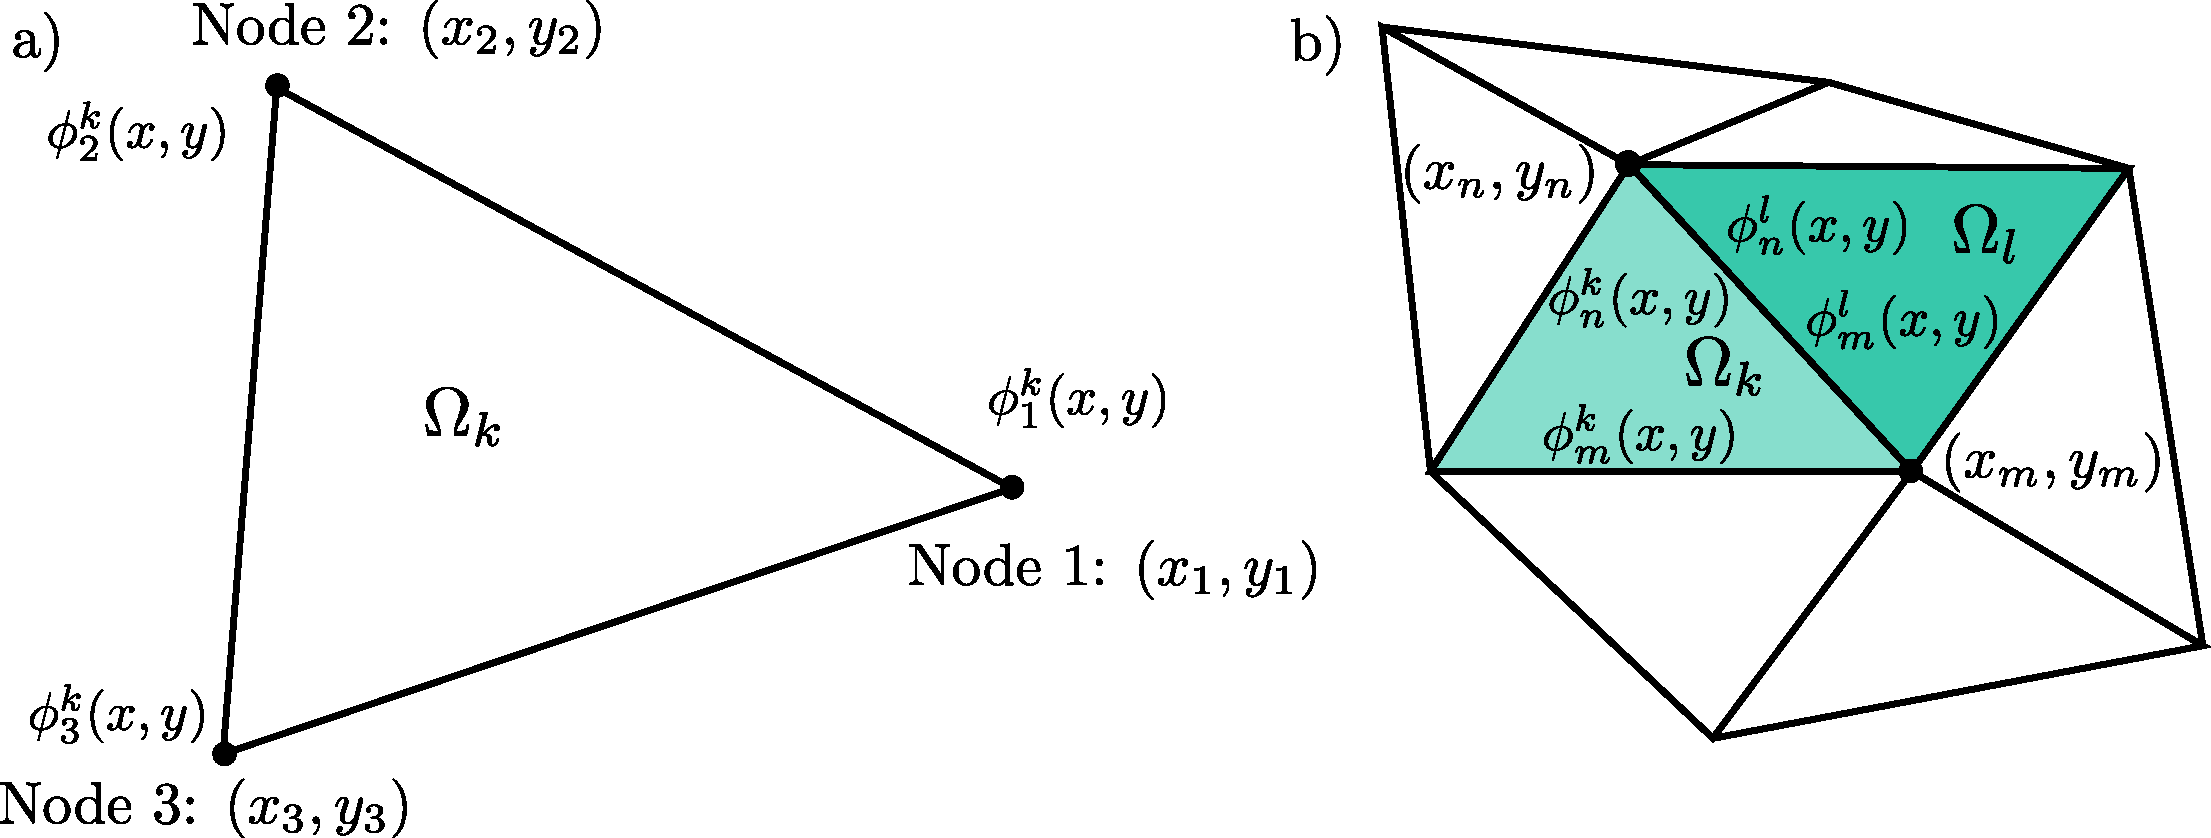
\includegraphics[width=\textwidth]{../figs/triangle.pdf}
\caption{a) A triangular element $\Omega_k$ of the domain together with the three vertices or nodes, each being the center of a FEM basis function $\phi$. Note that at each triangle, only three basis functions are nonzero, and each of them is affine over $\Omega_k$. b) Illustration of the triangulation. The basis functions centered at $(x_n, y_n)$ and $(x_m, y_m)$ overlap only in two triangular elements $\Omega_k$ and $\Omega_l$. Note that in both domains, the functions are affine but not the same as FEM basis functions are piecewise linear.}
\label{fig: triangles}
\end{figure}

The triangulation of the domain $\Omega = [0,1]\times[0,1]$ was done by using \texttt{pygmsh}, a python wrapper for the mesh generator tool Gmsh. Having constructed the triangular subdomains $\lbrace \Omega_k \rbrace_k$, construction of the required matrices can be achieved by integrating suitable functions over the subdomains. Integration over an arbitrary triangle can be done by a number of quadratures and was done in practice by utilizing \texttt{quadpy}, a python library for numerical integration.

The explicit formulas for the piecewise affine hat basis functions for each of the subdomains must be constructed to compute $T$, $V$ and $S$. Over the arbitrary subdomain $\Omega_k$ the relevant basis functions located at the vertices are given by

\begin{eqnarray}
\phi_1^k(x,y) &= \frac{1}{2A_k} \left[ (x_2y_3 - x_3y_2) + (y_2 - y_3)x + (x_3-x_2)y \right] \\
\phi_2^k(x,y) &= \frac{1}{2A_k} \left[ (x_3y_1 - x_1y_3) + (y_3 - y_1)x + (x_1-x_3)y  \right] \\
\phi_3^k(x,y) &= \frac{1}{2A_k} \left[ (x_1y_2 - x_2y_1) + (y_1 - y_2)x + (x_2-x_1)y \right]
\end{eqnarray}

where $A_k$ is the area of the triangle $\Omega_k$ and the labelling of the nodes and basis functions is as in Fig.~\ref{fig: triangles} a). These functions and their simple gradients are easily implemented by some modular arithmetic magic.

After defining a suitable potential function $V(x,y)$, we are ready to start constructing the matrices. Each of the matrices is of size $N \times N$, with row $i$ containing nonzero elements on all columns $j$ if there exists an edge connecting nodes $i$ and $j$, i.e. if the basis functions $\phi_i$ and $\phi_j$ overlap. The value of each of the nonzero elements is the sum of the integral of the relevant functions over the two (or, on the boundary, just one) common triangular subdomains. See Fig.~\ref{fig: triangles} b) and the colored relevant subdomains. Computing the integrals in Eq.~(\ref{eq: readyFEMeq}) and carefully inserting them into the matrices, we are left with all the pieces needed to solve the generalized eigenvalue problem in Eq.~(\ref{eq: matrixFormFEMeq}).

\begin{figure}[H]
\centering
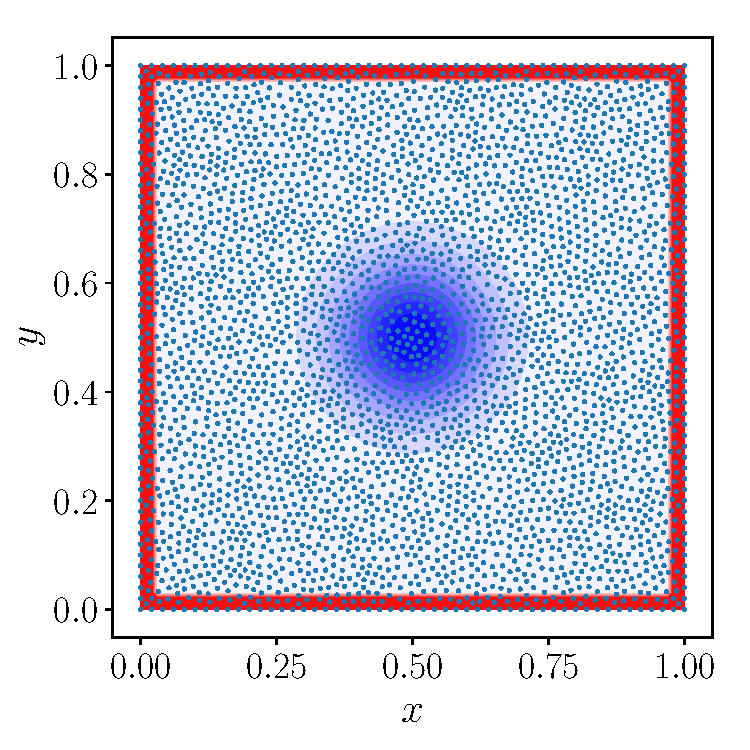
\includegraphics[width=0.5\textwidth]{../figs/pot.pdf}
\caption{The potential landscape used in initial tests of the FEM solver. The blue region in the middle is the Gaussian potential minimum and the red region is a high potential barrier approximating an infinite potential well. The blue dots are the triangulation nodes for $N=3436$. }
\label{fig: gaussPot}
\end{figure}


\begin{figure}[H]
\centering
\vspace{-5cm}
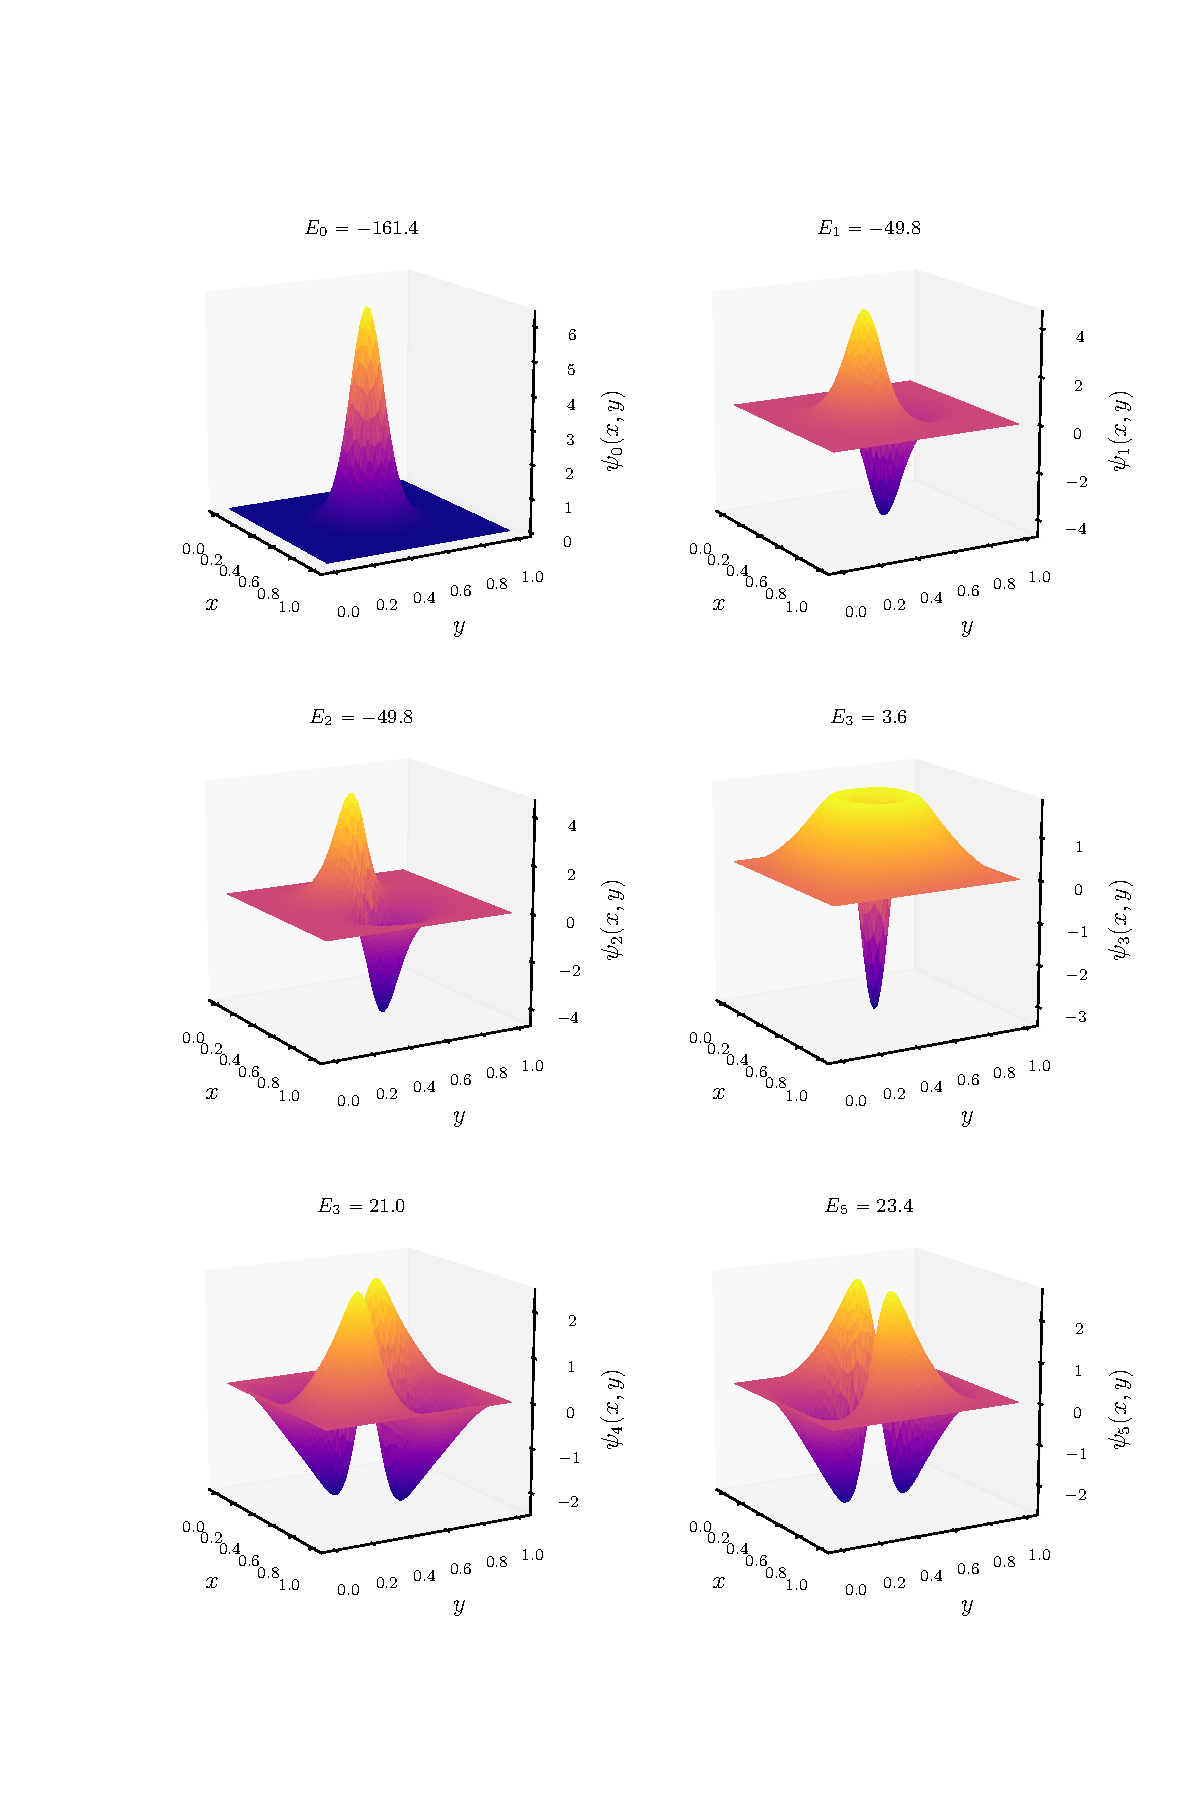
\includegraphics[width=\textwidth]{../figs/eigenfuncs_gauss.pdf}
\caption{The six lowest-energy eigenstates in the Gaussian potential well with $N=3436$. Note that it seems based on our FEM solution that only three of the states are bound to the potential minimum. Notice also the near-degenerate state pairs $(\psi_1, \psi_2)$ and $(\psi_4, \psi_5)$.}
\label{fig: gaussEigFuncs}
\end{figure}


\begin{figure}[H]
\centering
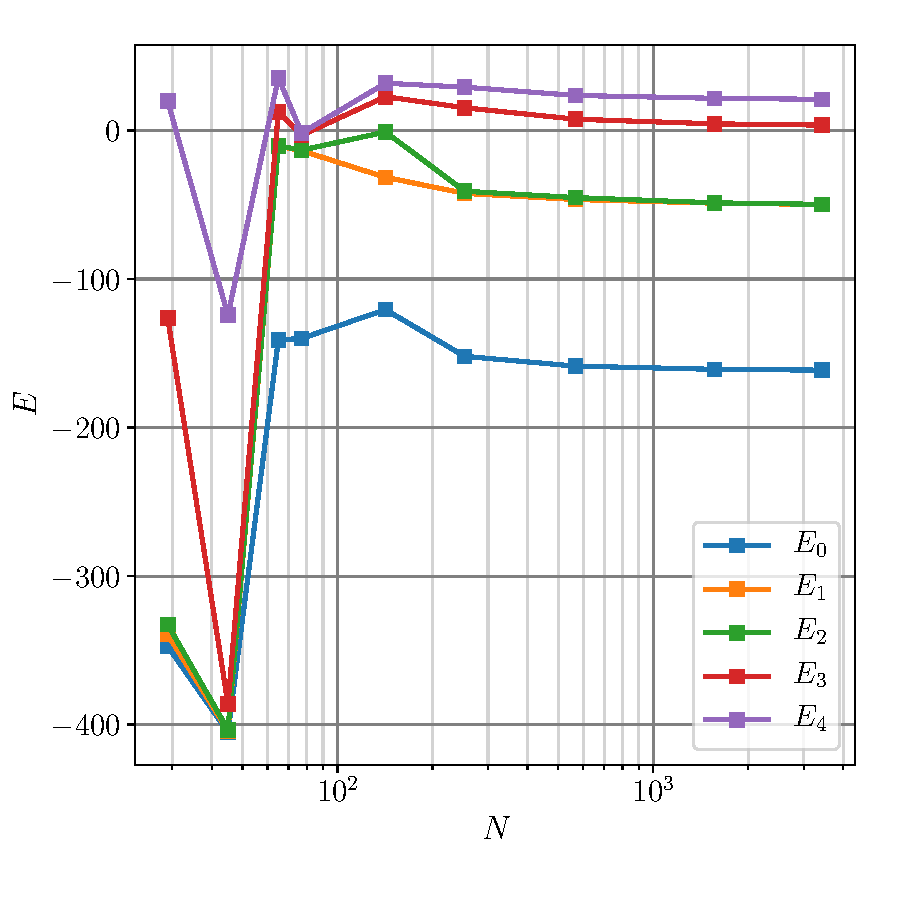
\includegraphics[width=0.7\textwidth]{../figs/energy_convergence.pdf}
\caption{The convergence of the energy eigenvalues as the FEM basis dimension $N$ increases.}
\label{fig: gaussEigVals}
\end{figure}



%\begin{figure}[h]
%\centering
%\begin{subfigure}[b]{.5\textwidth}
%  \centering
%  \includegraphics[width=\textwidth]{figs/wave_euler_forward.pdf}
%  \caption{Implicit Euler}
%  \label{fig:sub1}
%\end{subfigure}%
%\begin{subfigure}[b]{.5\textwidth}
%  \centering  
%  \includegraphics[width=\textwidth]{figs/wave_cn_forward.pdf}
%  \caption{Crank-Nicolson}
%  \label{fig:sub2}
%\end{subfigure}
%\caption{The results for the two integration schemes for forward time integration of the wave equation from $t_0=0$ to $t_{f}$ = 0.2}
%\label{fig:waveForward}
%\end{figure}



\end{document}
